\documentclass{article}
\usepackage[utf8]{inputenc}
\usepackage{amsmath}
\usepackage{amssymb}
\usepackage{graphicx}
\usepackage[margin = 1 in]{geometry}



\title{CS5220: Matrix Multiply Project}
\author{Junyoung Lim, Max Ruth, Arjun Sharma}
\date{October 5, 2020}

\begin{document}

\maketitle

\section{Introduction}
As a group, we have tried a variety of ways to optimize matrix-matrix multiplication. We have found that improvements to our code have followed a couple of rules. 

First, copying large amounts is bad. For instance, as a form of copy optimization, we attempted to copy the whole of \texttt{A}, \texttt{B}, and \texttt{C} into structured aligned arrays. However, any potential improvement due to alignment was negated by the large amount of time moving memory. With more careful timing and storage, it is likely that alignment could be used to effect, but it would take much more attention to detail than simple copying. Another option would be to use the specific commands allowed by the Intel compiler, shown in the \texttt{kdgemm.c} example.

Second, large improvements in the flop rate could be made with simple changes to the code and compiler. For instance, after the addition of three compiler flags, changing the loop order of the basic code, and adding the \texttt{restrict} keyword, the speed of the code improved by approximately an order of magnitude, especially for small matrices. However, when we tried writing large amounts of code (e.g., when trying the copy optimization previously described), the performance tended to go down. 




References: 

https://stackoverflow.com/questions/38190006/matrix-multiplication-why-non-blocked-outperforms-blocked

https://suif.stanford.edu/papers/lam-asplos91.pdf


\section{Discussion: Compilation Details}
The simplest design decisions that we made were on the compiler side. We used the GCC 8.3.0 compiler that was downloaded by default in the \texttt{build-essential} package. The three flags that we used for the compilation are the following:
\begin{itemize}
	\item \texttt{-O3} --- Enable more aggressive optimization than the flag \texttt{-O2} used by default. 
	\item \texttt{-ffast-math} --- Allows the compiler to reorder operations that may not actually be associative. We did not see a dramatic increase in the error of the result using this flag, although there would be a chance for that when floating point operations are seen as associative. Perhaps for more pathological matrix examples, we might have to worry about this flag.
	\item \texttt{-march=native} --- Optimizes the code for the specific machine architecture. When running on a desktop with the flag \texttt{-fopt-info-vec}, adding \texttt{-march=native} changed the vectorization from 16 bytes to 32 bytes wherever possible - allowing a potential doubling of the computation speed.
\end{itemize}

Of course, there are likely many more compiler options that could have been considered. Our group did not experiment with the CLang, gfortran, or Intel compilers. From the 


\section{Discussion: the Inner Kernel}
Plot: restrict vs. not restrict




\subsection{The \texttt{restrict} Keyword}
\begin{figure}
    \centering
    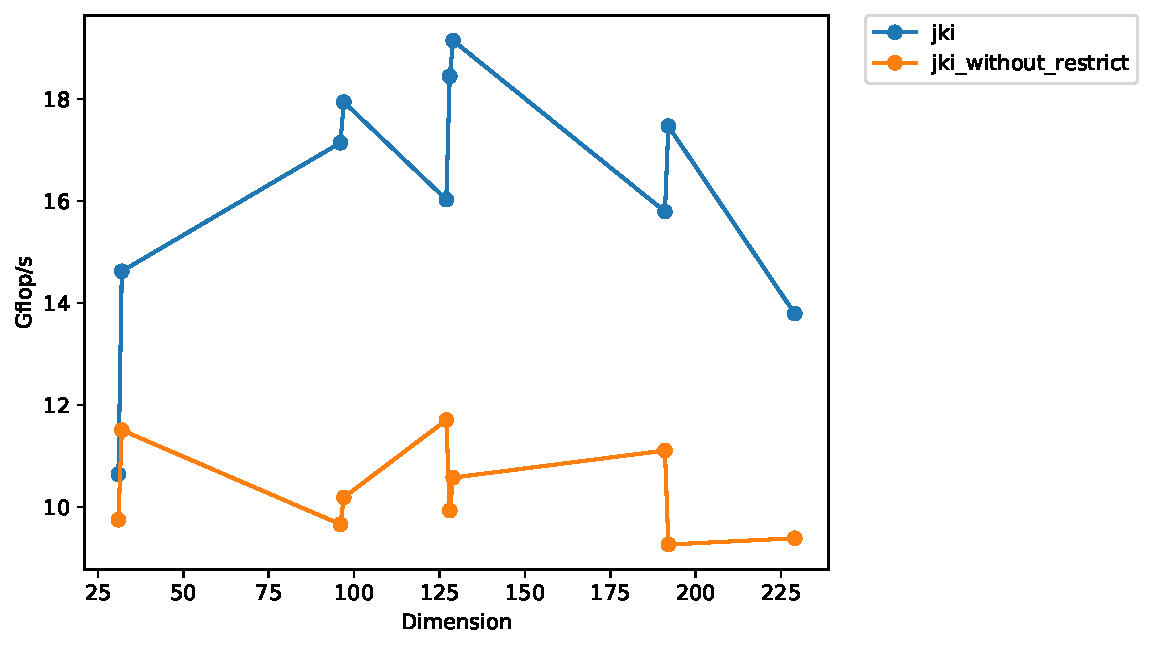
\includegraphics[width=0.8\columnwidth]{Restrict.pdf}
    \caption{Flop rates with and without the \texttt{restrict} keyword.}
    \label{fig:Restrict}
\end{figure}



\subsection{Loop Order}
\begin{figure}
    \centering
    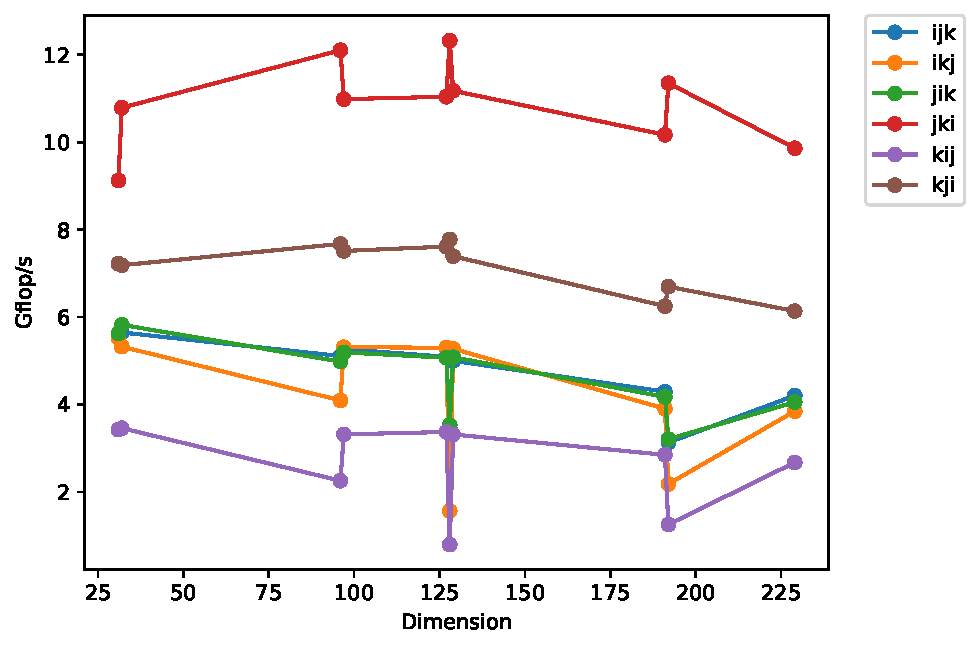
\includegraphics[width=0.8\columnwidth]{LoopOrder.pdf}
    \caption{Flop rates for each of the six possible loop orders for the kernel.}
    \label{fig:LoopOrder}
\end{figure}

Plot: All loop orders


\section{Discussion: Blocking Strategies}
- Helps with associative cache
\subsection{Blocking}


%\section{Discussion: Memory management}

%\subsection{Copy Optimization}
% - free memory







\section{Conclusion}
\begin{itemize}
	\item We should have more carefully profiled our code. 
	\item Specific details about what is happening on a computer are important.
	\item BLAS is impressive, but weirdly slow for small matrices.
	\item Alignment is confusing
\end{itemize}



\end{document}